\section{Interfacing the thermistor from \scilab}
\subsection{Interfacing the thermistor}
In this section we will explain a \scilab\ script to read the thermistor
values. Based on the acquired values, we will change
the state of the buzzer.  The shield has to be attached to the \arduino\ board
before doing these experiments and the \arduino\ needs to be connected to the computer
with a USB cable, as shown in \figref{arduino}.
The reader should go through the instructions given in
\secref{sec:sci-start} before getting started.

% The {\tt cmd\_analog\_in} command
% will be used to read from thermistor connected to an analog input
% pin. The experiments will be carried out using \scilab.

\begin{enumerate}
  \item In the first experiment, we will read the thermistor values and display it in
        \scilab\ Console. The code for this experiment is
        given in \sciref{sci:therm-read}. As explained earlier in \secref{sec:light-sci},
        we begin with serial port initialization. Then, we read the input coming from
        analog pin 4 using the following command:
        \lstinputlisting[firstline=4,lastline=4]
        {\LocTHERMscicode/therm-read.sce}
        Note that the one leg of the thermistor on
        the shield is connected to analog pin 4 of \arduino\,
        as given in \figref{fig:therm-conn}. The read value is stored in variable {\tt val} and
        displayed in the \scilab\ Console by the following command:
        \lstinputlisting[firstline=5,lastline=5]
        {\LocTHERMscicode/therm-read.sce} where {\tt val} contains
        the thermistor values ranging from 0 to 1023. The changes in
        the thermistor resistance is sensed as a voltage change between 0 to
        5V. The ADC maps the thermistor voltage readings in to values
        ranging from 0 to 1023. This means 0 for 0 volts and 1023 for 5
        volts. At room temperature you may get the
        output of ADC around 500. If a heating or cooling source is available,
        one can observe the increase or decrease in the ADC output. To
        encourage the user to have a good hands-on, we run these commands in
        a {\tt for} loop for 20 iterations.

        While running this experiment,
        the readers should try holding (or rubbing) the thermistor with their fingertips.
        Doing so will transfer heat from the person holding the
        thermistor, thereby raising the temperature of the thermistor. Accordingly, they should observe the change in the thermistor
        values on \scilab\ Console.


        % In the first experiment, \sciref{sci:therm-read} is used to read
        %   values from thermistor. First the serial port is opened using the
        %   command {\tt open\_serial} and passing the correct port number to
        %   it. The command {\tt cmd\_analog\_in} is used to read from the
        %   analog pin. The pin number is passed to this command as an
        %   argument. The read value is stored in some variable. The value is
        %   then displayed on the scilab console. A sleep of 500 millisecond is
        %   executed using the {\tt sleep} command and then the reading process
        %   is repeated 20 times by putting it in a {\tt for} loop. After the
        %   loop is finished the serial port is closed using the {\tt
        %     close\_serial} command.

  \item This experiment is an extension of the previous
        experiment. Here, we will use a \scilab\ script to
        turn a buzzer on using the thermistor values. This experiment
        can be considered as a simple fire alarm circuit that
        detects fires based on a sudden change in temperature and
        activates the buzzer.

        The program for this is available at
        \sciref{sci:therm-buzzer}.  As explained earlier,
        the ADC maps the thermistor voltage readings in to values
        ranging from 0 to 1023. This means 0 for 0 volts and 1023 for 5
        volts. In this experiment we compare the ADC output value with a user-defined
        threshold, which has been set as 550 in this experiment. One may note that
        this threshold would vary according to the location and time of performing
        this experiment. Accordingly, the readers are advised to change this threshold
        in \sciref{sci:therm-buzzer}. For testing purposes, one may note the
        normal thermistor readings generated from the execution of \sciref{sci:therm-read}
        and set a threshold that is approximately 10 more than these readings.

        In this experiment, as soon as the value exceeds 550, the buzzer is turned on. The following lines of code perform this
        comparison and sending a {HIGH} signal to digital pin 3 on \arduino:
        \lstinputlisting[firstline=6,lastline=10]{\LocTHERMscicode/therm-buzzer.sce}
        A delay of half a second is introduced
        before the next value is read. While running this experiment,
        the readers should try holding (or rubbing) the thermistor with their fingertips.
        Doing so will transfer heat from the person holding the
        thermistor, thereby raising the temperature of the thermistor.
        Accordingly, they should observe whether the threshold of 550 is achieved
        and the buzzer is enabled.

        \paragraph{Note:} Once the thermistor value reaches 550 (the threshold), the value will remain the same
        (unless it is cooled). Therefore, the buzzer will continuously produce the sound, which might be
        a bit annoying. To get rid of this, the readers are advised to
        execute some other code on \arduino\ like \sciref{sci:therm-read}.
\end{enumerate}


\begin{exercise}
  Carry out the exercise below: Convert the ADC output readings to
  degree Celsius. There are two ways to do so.
  \begin{enumerate}
    \item  In the first method,
          \begin{align}
            \frac{1}{T}=A+B*\ln(R)+C*(\ln(R))^3
            \label{therm-abc}
          \end{align}
          equation \ref{therm-abc} can be used if the value of A, B, C and R are
          known. The temperature T is in kelvin and thermistor resistance R is
          in ohms. The values of A, B and C can be found out by measuring
          thermistor resistance against three known values of temperatures. The
          values of temperature must be within the operating range and should
          typically include the room temperature. Once a set of three values of
          T and R are known it will result in three equations with three
          unknowns. The values of A, B, C can be found out by solving the three
          equations simultaneously. Once the values of A, B, C are known, the
          same equation can be used to directly convert resistance to kelvin. It
          can be then converted to Celsius. This method is preferred when the
          temperature coefficient of thermistor is not known or is known very
          approximately. This method is bit cumbersome but can give accurate
          temperature conversion.

    \item In the second method,
          \begin{align}
            \frac{1}{T}=\frac{1}{T_0}+\frac{1}{\beta}*\ln\left(\frac{R}{R_0}\right)
            \label{therm-beta}
          \end{align}
          equation \ref{therm-beta} can be used if the value of $\beta$ i.e. the
          Temperature Coefficient of Resistance of the thermistor used is
          known. The value of $\beta$ can be found in the data sheet of the
          thermistor used. $R$ is the resistance of thermistor at temperature
          $T$ in kelvin.  $R_0$ is the resistance of thermistor at room
          temperature $T_0$ in kelvin.
  \end{enumerate}
\end{exercise}

\subsection{Scilab Code}
\label{sec:therm-scilab-code}
\addtocontents{cod}{\protect\addvspace{\codclr}}

\begin{scicode}
  \ccaption{Read and display the thermistor values} {Read and display
    the thermistor values.  Available at
    \LocTHERMscibrief{therm-read.sce}.}
  \label{sci:therm-read}
  \lstinputlisting{\LocTHERMscicode/therm-read.sce}
\end{scicode}

\begin{scicode}
  \ccaption{Turning the buzzer on using thermistor values}
  {Turning the buzzer on using the thermistor values read by
    ADC.  Available at \LocTHERMscibrief{therm-buzzer.sce}.}
  \label{sci:therm-buzzer}
  \lstinputlisting{\LocTHERMscicode/therm-buzzer.sce}
\end{scicode}

\section{Interfacing the thermistor from Xcos}
In this section, we discuss how to read and use the thermistor values using
Xcos blocks. The reader should go
through the instructions given in \secref{sec:xcos-start} before
getting started.

\begin{enumerate}
  \item First we will read the thermistor values and display it.  When the
        file required for this experiment is invoked, one gets the GUI as in
        \figref{fig:therm-read}.  In the caption of this figure, one
        can see where to locate the file.

        As discussed in earlier chapters, we start with the initialization
        of the serial port. Next, using {\tt Analog Read} block, we read
        the values of thermistor connected on analog pin 4.
        Next, we use a scope to plot the values
        coming from this pin. When this Xcos file is simulated,
        a plot is opened, as shown in \figref{fig:therm-read-output}.

        \begin{figure}
          \centering
          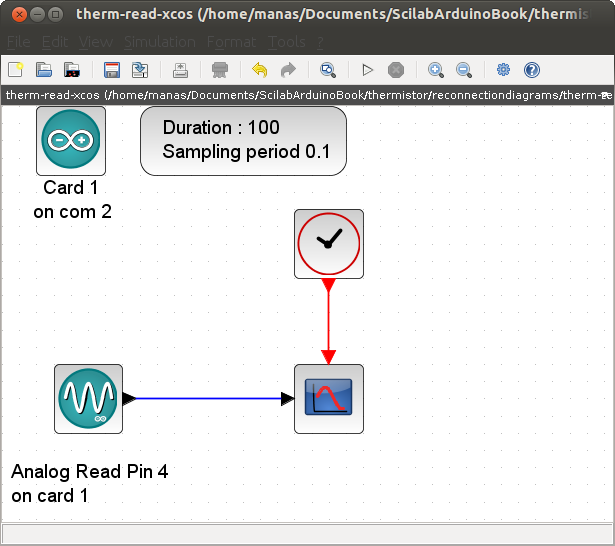
\includegraphics[width=\smfigp]{\LocTHERMfig/therm-read-xcos.png}
          \caption[Xcos diagram to read thermistor values]{Xcos diagram to
            read thermistor values.  This is what one sees when
            \LocTHERMscibrief{therm-read.zcos}, is invoked.}
          \label{fig:therm-read}
        \end{figure}

        We will next explain how to set the parameters for this simulation.
        To set value on any block, one needs to right click and open the
          {\tt Block Parameters} or double click.  The values for each block
        is tabulated in \tabref{tab:therm-read}.  All other parameters are to
        be left unchanged.
        \begin{table}
          \centering
          \caption{Xcos parameters to read thermistor}
          \label{tab:therm-read}
          \begin{tabular}{llc} \hline
            Name of the block & Parameter name             & Value     \\ \hline
            ARDUINO\_SETUP    & Identifier of Arduino Card & 1         \\
                              & Serial com port number     & 2\portcmd \\ \hline
            TIME\_SAMPLE      & Duration of acquisition(s) & 100       \\
                              & Sampling period(s)         & 0.1       \\ \hline
            ANALOG\_READ\_SB  & Analog Pin                 & 4         \\
                              & Arduino card number        & 1         \\ \hline
            CSCOPE            & Ymin                       & 200       \\
                              & Ymax                       & 600       \\
                              & Refresh period             & 100       \\ \hline
            CLOCK\_c          & Period                     & 0.1       \\
                              & Initialisation Time        & 0         \\ \hline
          \end{tabular}
        \end{table}
        \begin{figure}
          \centering
          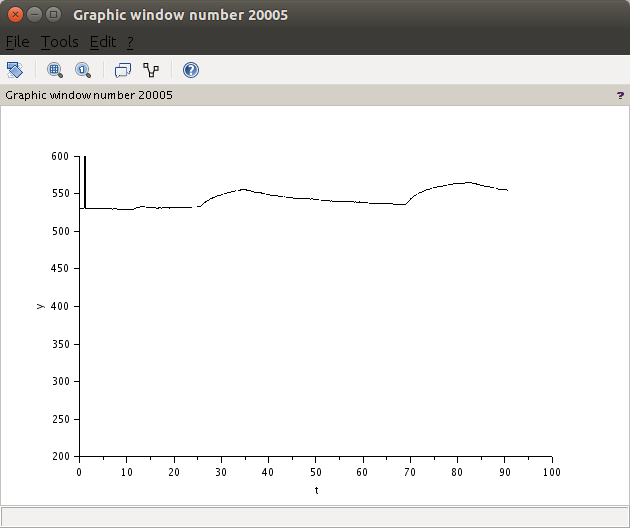
\includegraphics[width=\smfigp]{\LocTHERMfig/therm-read.png}
          \caption{Plot window in Xcos to read thermistor values}
          \label{fig:therm-read-output}
        \end{figure}

        While running this experiment,
        the readers should try holding (or rubbing) the thermistor with their fingertips.
        Doing so will transfer heat from the person holding the
        thermistor, thereby raising the temperature of the thermistor. Accordingly, they should observe the change in the thermistor
        values in the output plot, as shown in \figref{fig:therm-read-output}.

  \item In the second experiment, we will switch on a buzzer
        depending on the thermistor readings (ADC output).
        When the file required for this
        experiment is invoked, one gets the GUI as in \figref{fig:therm-buzzer}.
        In the caption of this figure, one can see where to locate the file.

        \begin{figure}
          \centering
          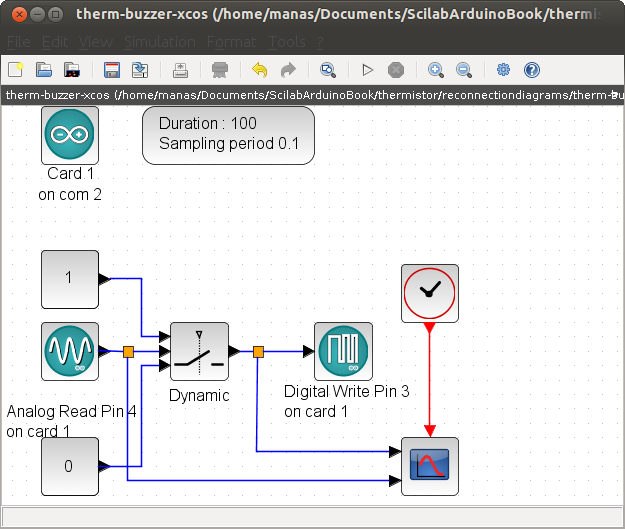
\includegraphics[width=\lgfig]{\LocTHERMfig/therm-buzzer-xcos.png}
          \caption[Xcos diagram to read the value of thermistor, which is
            used to turn the buzzer on] {Xcos diagram to read the value
            of the thermistor, which is used to turn the buzzer on.
            This is what one sees when
            \LocTHERMscibrief{therm-buzzer.zcos}, is invoked.}
          \label{fig:therm-buzzer}
        \end{figure}

        We will next explain how to set the parameters for this simulation.
        To set value on any block, one needs to right click and open the
          {\tt Block Parameters} or double click.  The values for each block
        is tabulated in \tabref{tab:therm-buzzer}.  In the CSCOPE\_c block, the
        two values correspond to two graphs, one for digital write and other
        for analog read values. All other parameters are to be left
        unchanged. When this Xcos file is simulated, a plot is opened,
        as shown in \figref{fig:therm-buzzer-output}.

        \begin{table}
          \centering
          \caption{Xcos parameters to read thermistor and switch the buzzer}
          \label{tab:therm-buzzer}
          \begin{tabular}{llc} \hline
            Name of the block  & Parameter name             & Value     \\ \hline
            ARDUINO\_SETUP     & Identifier of Arduino Card & 1         \\
                               & Serial com port number     & 2\portcmd \\ \hline
            TIME\_SAMPLE       & Duration of acquisition(s) & 100       \\
                               & Sampling period(s)         & 0.1       \\ \hline
            ANALOG\_READ\_SB   & Analog pin                 & 4         \\
                               & Arduino card number        & 1         \\ \hline
            CMSCOPE            & Ymin                       & 0 300     \\
                               & Ymax                       & 1 600     \\
                               & Refresh period             & 100 100   \\ \hline
            CLOCK\_c           & Period                     & 0.1       \\
                               & Initialisation time        & 0         \\ \hline
            SWITCH2\_m         & Datatype                   & 1         \\
                               & threshold                  & 550       \\
                               & pass first input if field  & 0         \\
                               & use zero crossing          & 1         \\ \hline
            DIGITAL\_WRITE\_SB & Digital pin                & 3         \\
                               & Arduino card number        & 1         \\ \hline
          \end{tabular}
        \end{table}

        \begin{figure}
          \centering
          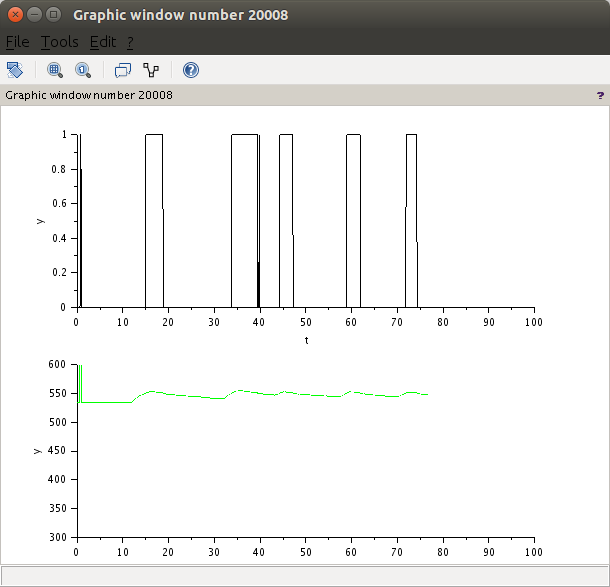
\includegraphics[width=\lgfig]{\LocTHERMfig/therm-buzzer.png}
          \caption{Plot window in Xcos to read thermistor values and the state of LED}
          \label{fig:therm-buzzer-output}
        \end{figure}

        While running this experiment,
        the readers should try holding (or rubbing) the thermistor with their fingertips.
        Doing so will transfer heat from the person holding the
        thermistor, thereby raising the temperature of the thermistor.
        Accordingly, they should observe whether the threshold of 550 is achieved
        and the buzzer is enabled.

        \paragraph{Note:} Once the thermistor value reaches 550 (the threshold), the value will remain the same
        (unless it is cooled). Therefore, the buzzer will continuously produce the sound, which might be
        a bit annoying. To get rid of this, the readers are advised to
        execute some other code on \arduino\ like the Xcos file shown in
        \figref{fig:therm-read}.
\end{enumerate}


